\subsubsection{The Design of the OmniBot}
\label{sec:omnibot_design}

By leveraging a new propulsion method for land and water locomotion in conjunction with quad-rotor designs for flight, coupled with a waterproof hull and buoyancy control unit to alter its density, the OmniBot is able to travel on and through water, over land, and in the air. As far as we know, the OmniBot constitutes the first robot that could cover all four typical kinds of environments.

Covering all four mentioned domains presents a special challenge that is more than combining parts. As stated, there exist robotic solutions for each or a couple of domains, however, each has requirements or solutions that can be at odds with the requirements of a different domain. 

We break these challenges into the locomotive and structural aspects, where locomotive covers the means by which the Omnibot is to move itself through a given media and structural covers the physical properties the platform has to deal with the 4 kinds of regions. 
  
\subsubsection{Locomotion}

Central to the functionality and usability of a mobile robotic platform is the methods by which it moves itself through the environment it is in. Often, aforementioned methods amounts to be a fundamental choice as it places constraints on battery life, feasible paths to be followed, and the type of terrain to be traversed, variables which are of critical importance to all mobile platforms with a limited supply of power. 

For the OmniBot, the screwdrive powertrain was chosen for its ability to traverse both land and water environments while a quad-rotor design was chosen for flight due to its stability, vertical-take-off-and-lift (VTOL), and hovering capabilities.  

\subsubsection{Screwdrive}

Screwdrive propulsion is a relatively neglected method of locomotion that has been shown to successfully propel military, scientific, and recreational vehicles across a wide variety of terrains ranging from snow to water and mud to sand \cite{Fales1972, Cole1961c, Dugoff1967}. However, most of this core research dates back to the 1960s and 1970s. A few modern exceptions are \cite{Freeberg2010} and \cite{Osinski2014}, where the former explores multi-screw drives and  the latter the modeling of a dual screw system. However, in the robotic community they are exceptional as screwdrives are by no means a popular form of locomotion. 

%%screwdrive
%\begin{figure}
  %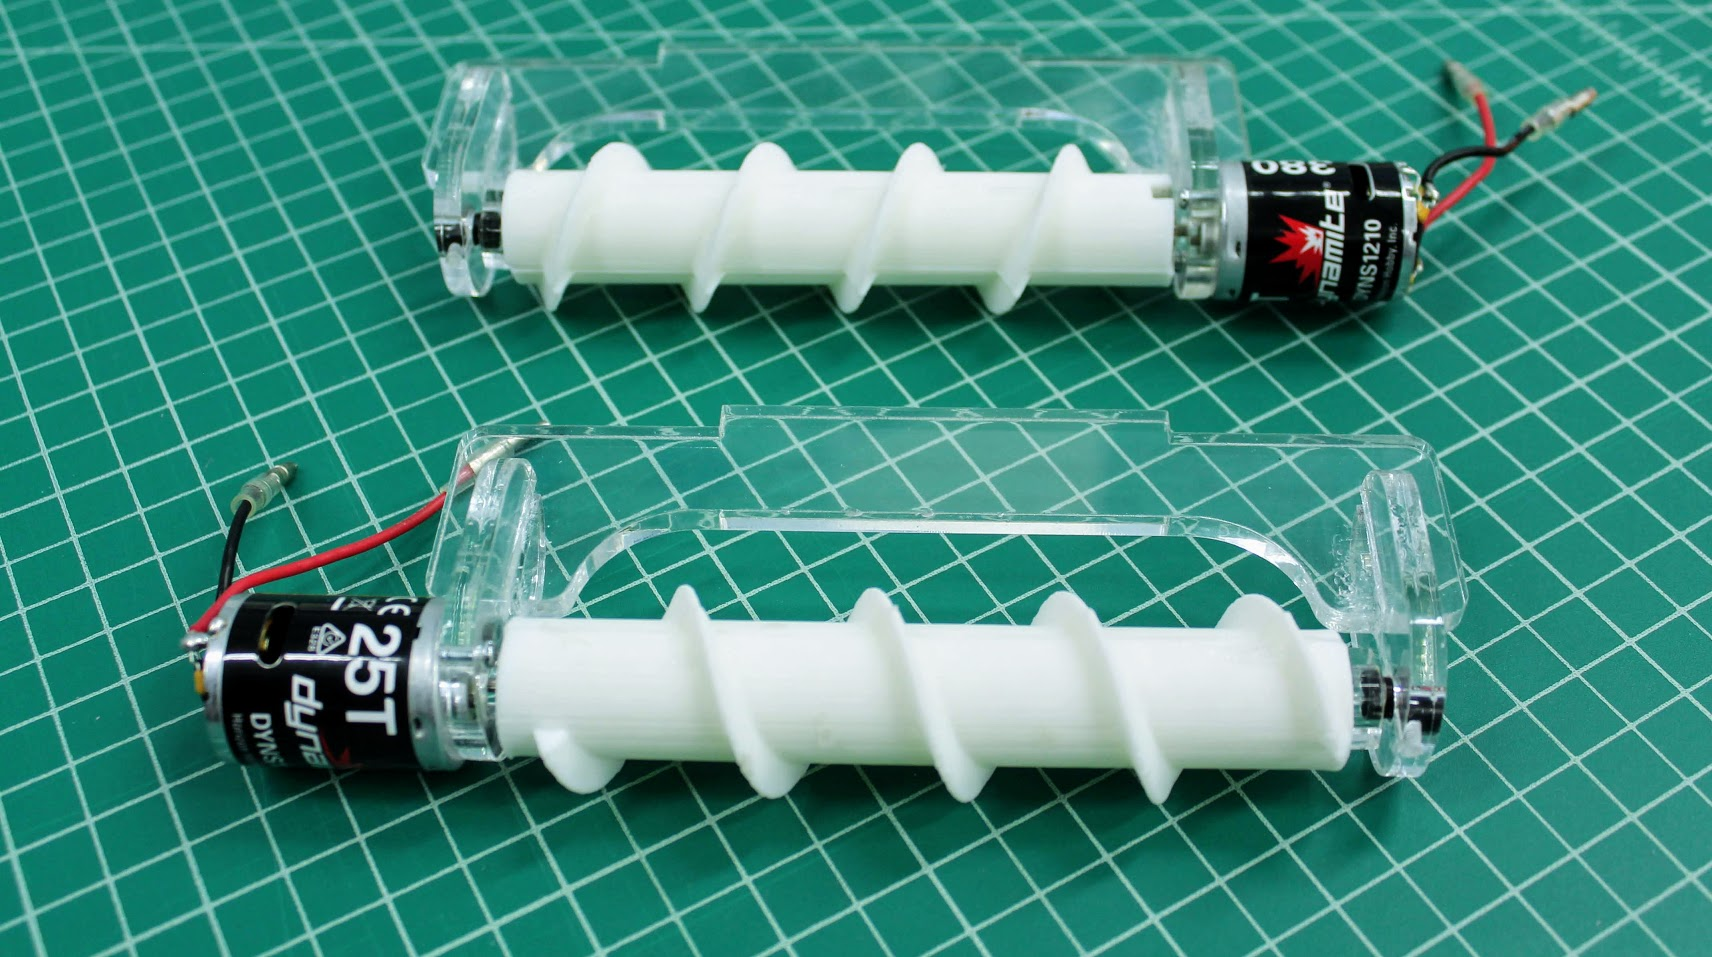
\includegraphics[width=\linewidth]{images/screwdrive.JPG}
  %\caption{The dual screwdrive}
  %\label{fig:screwdrive}
%\end{figure}

On the Omnibot a dual-parallel screw configuration is chosen, shown in Figure~\ref{fig:screwdrive}. It employs two independently actuated and contra-rotating continuous propellers. The screws consists of a cylinder with blades forming a helix around its surface. When rotated in a coordinated fashion, these allow a variety of movements. 

The screws provide a combination of tractive and rolling forces. The tractive forces are those created from the longitudinal displacement of material against the screw's helix. The rolling forces are the ones that result from the rotation of the cylinder about its axes. In Figure~\ref{fig:screw_FBD_alpha_0} two contra-rotating screws are shown.  

\emph{Rolling forces} are akin to those of the wheels on a vehicle. The wheels turn and, given enough friction with the surface it is rolling on, push the surface to provide movement in the same direction as the wheels are turning. 

\emph{Traction forces} as they have been called in \cite{Freeberg2010}, result from the blade of the screw digging into and pushing against material. In the case that the material is a solid, such as dirt or snow, then the screw propels itself forward in a manner similar to the \emph{rolling force} modality. On the other hand, if the material is a fluid, such as water, then the screw pushes the fluid in a direction and creates \emph{thrust}.

The inter-screw angle affects the direction in which the tractive and rolling forces are exerted. Furthermore, in systems with two independently actuated screws, the inter-screw angle affects the resulting motions from the net forces of the competing or cooperating screws. The redirection and interplay of the forces from the dual-screw set-up can be seen in Figure~\ref{fig:screw_FBD_alpha_0} and Figure~\ref{fig:screw_FBD_alpha_45} where the inter-screw angle is set to 0 and 45 degrees, respectively. 

Figure~\ref{fig:screw_FBD_alpha_0} shows the direction of the force when the blade is engaged. This mode is optimal for a screwdrive system because the direction of the force together with the independence of the actuators can be used to move the vehicle forward, backward, laterally, and to allow rotations in place, in effect, omnidirectional locomotion. 

\begin{figure}[ht]
	\centering
	\includegraphics[scale=0.25]{images/sd/screw_propulsion_FBD_alpha_0.pdf}
    \caption{Inter-screw angle of 0 degrees (parallel)}
	\label{fig:screw_FBD_alpha_0} 
\end{figure}

\begin{figure}[th]
	\centering
	\includegraphics[scale=0.25]{images/sd/screw_propulsion_FBD_alpha_45.pdf}
    \caption{Inter-screw angle of 45 degrees}
	\label{fig:screw_FBD_alpha_45} 
\end{figure}

\subsubsection{Thrusters}
A quad-copter design was chosen based on its ability to provide the amount of thrust necessary to lift the platform, its ability to offer VTOL, but most importantly because it allows effective air to ground and water transitions and vice versa, without impeding the other modes or transitions. 

The VTOL capabilities and controllability allow the robot to land carefully atop the screwdrive subsystem. Similarly, when transitioning from water the Omnibot was designed in such a way that the propellers are near the top of the robot and able to fly. Fixed-wing alternatives would have placed additional and incompatible restriction on weight, size, and other variables all while increasing the size. 


\subsubsection{Mechanical Design}

Most of the OmniBot's electronic parts are enclosed in a waterproof transparent sphere, making it easy to take off and land due to less friction. On the other hand, the transparency allows for cameras to be added inside as well. 

A removable payload “disc” around the globe can be used to extend the capabilities of the robot in various important ways. Different sensor suites will be mounted on the disk in such a way to allow easy deployment of many OmniBots with different payloads.

\subsubsection{Weight and Cost}

By integrating multiple mechanisms together, we have built a prototype, the weight of which is around 1.4 kg, and the cost is less than \$1,000 USDs. Therefore, it is cost-effective to deploy in different environments to test its capabilities.

\subsubsection{Density}

The buoyancy control unit works by ingesting water such as is the case in the Aquapod \cite{Carlson2011} and altering the robot's mass. Since the bladder is contained within a fixed volume, the density changes:

$$ \rho_{omnibot} = (mass_{omnibot}+mass_{bladder})/volume_{omnibot} $$ 

When the mass of the ingested media is enough to alter the OmniBot's density above that of the media it is contained in, it sinks. Reversing this process leads to the robot floating upwards towards the surface. 

$$ \rho_{omnibot} > \rho_{water} $$
$$ \frac{\rho_{omnibot}}{\rho_{water} } > 1 $$
$$ \rho_{water} = 1000 \frac{kg}{m^3} = 1 \frac{g}{cm^3} $$ 

\subsubsection{Sealing}
The main seal of the OmniBot consists of a face type seal employed between the two flanged hemispheres that comprise the main body of the robot. The hull halves squeeze an O-ring that is contained within a gland. This O-ring together with the gland provide protection for more than the equivalent of 5 meters of internal and external pressure. 

The numerous connections for the thrusters and screwdrive motors on the exterior of the robot are made through cable penetrators which also employ an elastomer to seal the interface where the surface is breached while allowing cables through. These are also removable by removing a nut, which is necessary for the maintainance of a field robot. 

\subsubsection{Electronics and Software}

The prototype is built by integrating many off-the-shelf parts together with self-designed components. In terms of electronic ones, we bought lightweight yet powerful rotors and electronic speed controllers (ESCs), made use of the latest version of the Pixhawk 4 platform \cite{pixhawkadmin_introducing_2018} and the PX4 flight stack \cite{noauthor_open_nodate} serves as our starting point, based on which we implement our own multipurpose platform control model.

The overall state machine model of the system is composed of an UAV, UGV, USV, and UUV, driving distinct propelling mechanisms according to their respective control algorithms.

\section{Experiments and Results}
\label{experiments_omnibot}

With the constructed model, we firstly tested it in each individual setting, then we verified that it can switch between different modes to adapt to different scenarios, as detailed below.

\subsubsection{In the Air}

Equipped with four light yet powerful rotors, OmniBot is able to fly up as a common quad-rotor drone. In Figure \ref{fig:omni_flight}, the OmniBot is taking off. 


\begin{figure}
  
\includegraphics[width=\linewidth]{images/omnibot_flight_2.PNG}
  \caption{The OmniBot is taking off}
  \label{fig:omni_flight}
\end{figure}

\subsubsection{On the Ground}

As seen from Figure \ref{fig:omnibot} when put on the ground, the robot can move around using two screw drives, which are especially suitable for exploration of sandy or muddy areas.

\subsubsection{On the Water Surface}

As seen from Figure \ref{fig:omnibot_on_water}, since the overall density of the OmniBot is less than the water, it can float in the water and move around thanks to the screwdrive mechanism.

\begin{figure}
  \includegraphics[width=\linewidth]{images/omnibot/omnibot_isoview.JPG}
  \caption{The OmniBot is under waterz}
  \label{fig:omni_submerge_top_view}
\end{figure}

\subsubsection{Under the Water}

By pumping water into the shell, the well-sealed OmniBot can dive into the water as well, as can be seen in Figure \ref{omnibot_submerge}.

\begin{figure}
  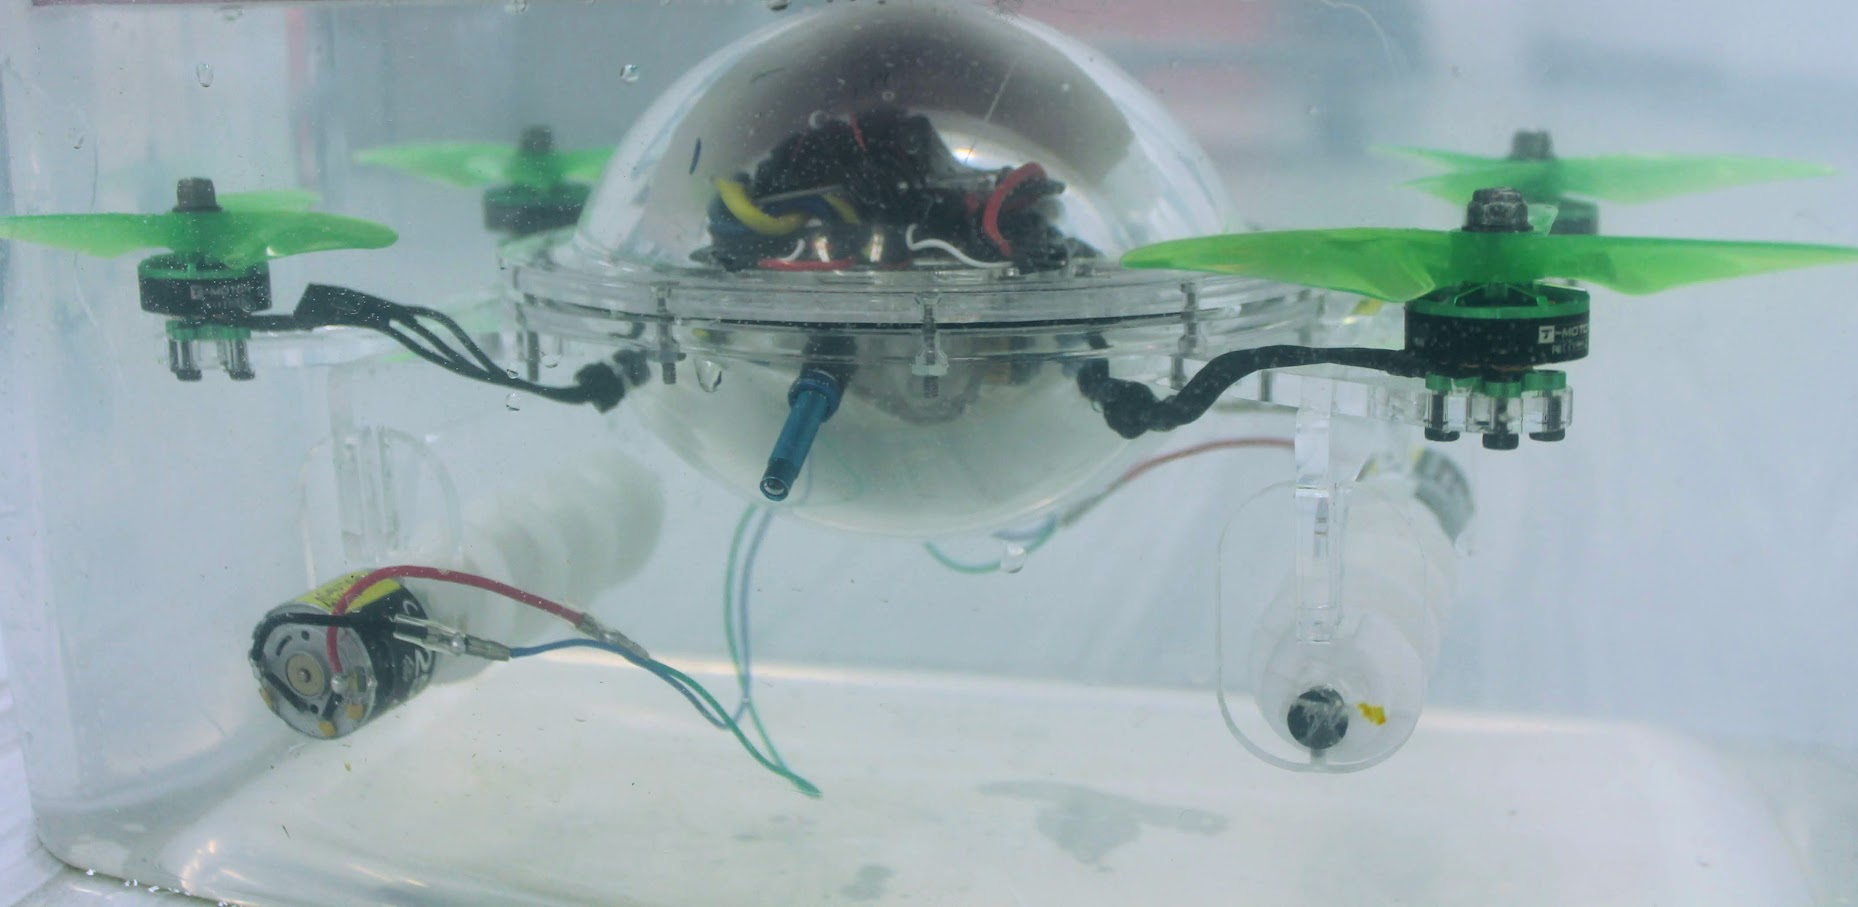
\includegraphics[width=\linewidth]{images/omnibot_submerged_back.JPG}
  \caption{The OmniBot is under water}
  \label{fig:omni_submerge_front_view}
\end{figure}

\subsubsection{Transitions Between Varying Modes}

After testing the OmniBot in each individual environment, we also verified its capability of adapting from one kind of active area to another. A detailed video has been uploaded to demonstrate transitions between air, land, and water. 

\section{Conclusions and Future Work}
\label{conclusion_future}

To further advance the competence of robotic platforms in diversified changing scenarios, we propose to construct a new model that can cover all of the four common environments that a robot may encounter, therefore making it possible to survive unforeseeable hazards.

Upon building a prototype, we tested it in different kinds of terrains and especially its ability to switch seamlessly among distinct modes. Experimental results demonstrate that the OmniBot is able to travel through four kinds of environments as expected.

Essentially, the OmniBot can serve as a common platform. Based on our current work, in the near future, we plan to make the OmniBot more intelligent by equipping it with various sensors for specific applications, such as crop monitoring on land and air, lake health evaluation from the air, surface, and in the water, search and rescue missions, etc.
